\chapter{Feature Detection and Matching}
\label{ch:lesson20}

This begins Part 2: classical 3D computer vision, where the algorithms increasingly work across \emph{multiple} images of a scene --- video frames, or several cameras --- rather than a single one. The first problem that creates: two images of the same scene rarely put the same content at the same pixel location, since rotation, scale, and viewpoint all shift things around. This chapter builds toward feature-based matching, which survives exactly those changes: first \textbf{corner detectors} (Harris, Shi-Tomasi) that find distinctive, repeatable points, then \textbf{SIFT}, which adds scale-invariance and a descriptor that can be matched between two different-looking images of the same scene.

\section{The structure tensor: what makes a good point to match?}

At each pixel, build the $2\times2$ \textbf{structure tensor} from the local window of gradients (Chapter~\ref{ch:lesson12}):
\begin{equation}
M = \sum_{\text{window}} \begin{bmatrix}I_x^2 & I_xI_y \\ I_xI_y & I_y^2\end{bmatrix}.
\end{equation}
This should look familiar: it's exactly the moment covariance matrix from Chapter~\ref{ch:lesson06}, but built from gradients instead of pixel coordinates. Its eigenvalues $\lambda_1\ge\lambda_2$ describe the local intensity structure: both small means a \textbf{flat} region (gradients weak in every direction), one large and one small means an \textbf{edge} (gradient strong perpendicular to it, weak along it), and both large means a \textbf{corner} (gradient strong in every direction --- exactly the kind of point that can be precisely relocalized in another image), as illustrated on a test image in Figure~\ref{fig:l20-1}.

\begin{figure}[h]
\centering
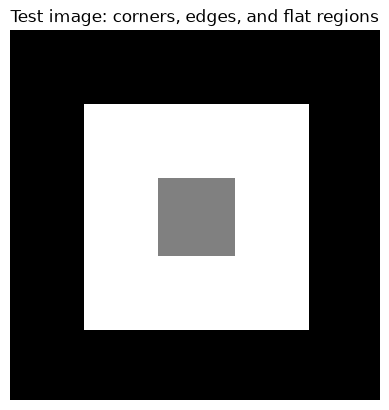
\includegraphics[width=0.3\textwidth]{figures/lesson20_fig01.png}
\caption{A test image containing corners, edges, and flat regions.}
\label{fig:l20-1}
\end{figure}

\section{Harris corner detector}

Directly computing eigenvalues everywhere is a bit expensive, so Harris and Stephens (\citelink{harrisstephens1988}{1988}) proposed a cheaper proxy using only $\det(M)$ and $\operatorname{trace}(M)$ (computable without ever finding eigenvalues):
\begin{equation}
R = \det(M) - k \cdot \operatorname{trace}(M)^2, \qquad k \approx 0.04.
\end{equation}
$R$ is large and positive at corners, negative at edges, and near zero on flat regions. A from-scratch implementation correlates perfectly ($1.0$) with \code{cv2.cornerHarris}, shown in Figure~\ref{fig:l20-2}.

\begin{figure}[h]
\centering
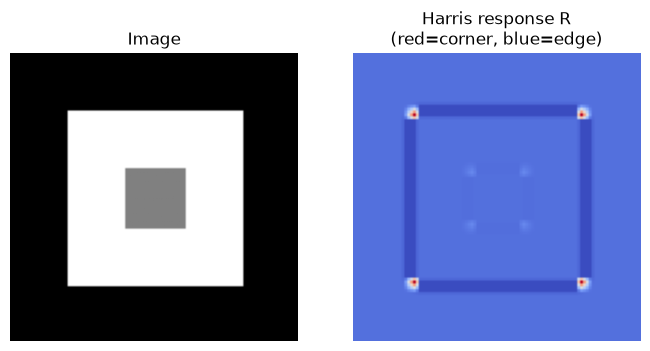
\includegraphics[width=0.7\textwidth]{figures/lesson20_fig02.png}
\caption{The test image and its Harris response $R$ (red = corner, blue = edge).}
\label{fig:l20-2}
\end{figure}

\section{Shi-Tomasi: ``Good Features to Track''}

Shi and Tomasi (\citelink{shitomasi1994}{1994}) argued for using the \textbf{minimum eigenvalue} of $M$ directly instead of Harris's determinant/trace proxy:
\begin{equation}
R_{\text{ST}} = \min(\lambda_1, \lambda_2).
\end{equation}
A point is only a strong corner if \emph{both} eigenvalues are large --- the minimum being large is exactly that condition, and (unlike Harris's $R$) it has a direct, easily interpretable meaning: it's proportional to the worst-case tracking precision in any direction. A from-scratch computation correlates perfectly ($1.0$) with \code{cv2.cornerMinEigenVal}, as Figure~\ref{fig:l20-3} shows.

\begin{figure}[h]
\centering
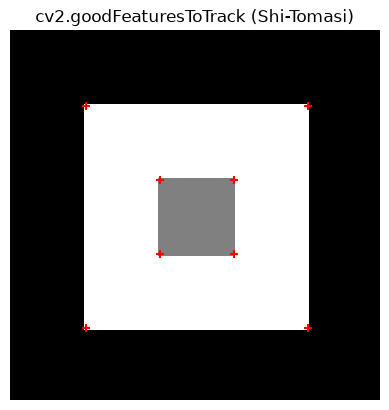
\includegraphics[width=0.3\textwidth]{figures/lesson20_fig03.png}
\caption{\code{cv2.goodFeaturesToTrack} (Shi-Tomasi) corners marked in red.}
\label{fig:l20-3}
\end{figure}

\section{The scale problem}

Harris and Shi-Tomasi both operate at a single, fixed window size. Zoom the same corner in or out, and it may stop looking like a corner at that fixed scale (a sharp corner becomes a gentle curve when zoomed out enough) --- these detectors are not scale-invariant. \textbf{SIFT} (Scale-Invariant Feature Transform) (\citelink{lowe2004}{Lowe, 1999/2004}) fixes this by searching for keypoints across an entire scale-space, not just one window size.

\section{SIFT: scale-space extrema and descriptors}

SIFT's pipeline, at a glance:
\begin{enumerate}
  \item Build a \textbf{Difference-of-Gaussians (DoG) scale-space} --- exactly the DoG approximation to the Laplacian from Chapter~\ref{ch:lesson13}, computed at many blur levels.
  \item Find keypoints as local extrema of DoG response across both space \emph{and} scale --- a point that's a maximum compared to its 26 neighbors (8 in the current scale, 9 in each scale level up and down).
  \item Assign each keypoint a dominant orientation from the local gradient histogram, so descriptors can be made rotation-invariant.
  \item Build a 128-dimensional descriptor from histograms of gradient orientations in a $4\times4$ grid of subregions around the keypoint.
\end{enumerate}
The result: a keypoint with a position, a scale, an orientation, and a descriptor vector designed to be very similar between two images even under moderate rotation, scaling, and illumination change. On a real photo, \code{cv2.SIFT\_create()} finds $723$ keypoints, each with a 128-dim descriptor, shown in Figure~\ref{fig:sift-keypoints}.

\begin{figure}[h]
\centering
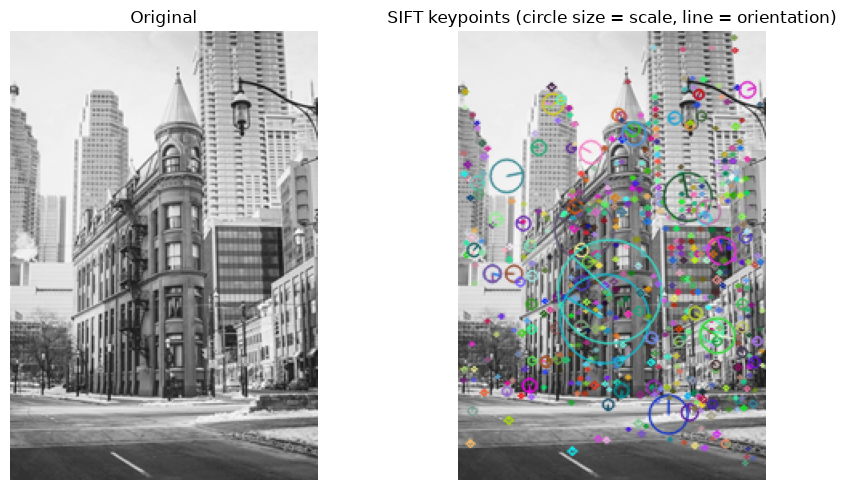
\includegraphics[width=0.9\textwidth]{figures/lesson20_fig04.png}
\caption{SIFT keypoints overlaid on the original (circle size = scale, line = orientation). \attrib{Photo by \href{https://unsplash.com/@dawsonlovell}{Dawson Lovell} on \href{https://unsplash.com/photos/flatiron-building-in-toronto-W_MUqtuHwyY}{Unsplash}.}}
\label{fig:sift-keypoints}
\end{figure}

\section{Matching under rotation and scale}

Rotating and shrinking the image with a \emph{known} transform ($35^\circ$ rotation, $0.7\times$ scale), detecting SIFT features independently in both, and matching descriptors with a nearest-neighbor search: $723$ keypoints in the original, $365$ in the rotated-and-scaled version. \textbf{Lowe's ratio test} keeps a match only if the best candidate is meaningfully closer than the \emph{second}-best candidate --- a simple, effective way to reject ambiguous matches; here it keeps $191$ of $723$ candidate pairs.

\subsection*{How many matches are actually correct?}

Because the exact transform used to create the second image is known, each matched keypoint can be mapped through it and checked directly against where it was actually matched: $175$ of the $191$ ratio-test survivors ($92\%$) are geometrically correct (Figure~\ref{fig:l20-5}).

\begin{figure}[h]
\centering
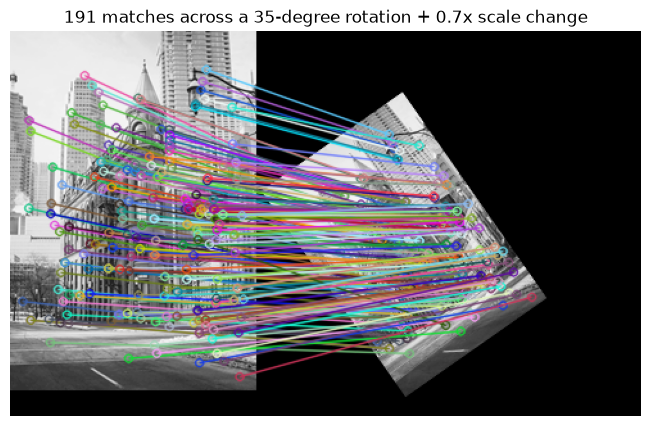
\includegraphics[width=0.95\textwidth]{figures/lesson20_fig05.png}
\caption{$191$ matches across a $35^\circ$ rotation $+$ $0.7\times$ scale change. Nearly all the ratio-test survivors are genuinely correct correspondences, despite the rotation and scale change --- something a detector fixed to one scale and orientation simply couldn't recover.}
\label{fig:l20-5}
\end{figure}

This is exactly what makes SIFT-style features the classic approach for tasks like image stitching, object recognition, and visual localization.

\subsection*{Exercises}
\begin{enumerate}
  \item Increase the rotation angle to $90^\circ$ and the scale to $0.3$. Does the number of good matches and the geometric-correctness percentage hold up, or degrade? At what point does SIFT start to struggle?
  \item Try \code{cv2.ORB\_create()} (a much faster, free binary-descriptor alternative to SIFT) with \code{cv2.NORM\_HAMMING} in the \code{BFMatcher} instead of the default L2 norm. Compare the number of good matches and qualitatively compare speed using \code{\%timeit} on \code{detectAndCompute}.
  \item Lower the ratio-test threshold from $0.75$ to $0.6$. How do the number of good matches and the fraction that are geometrically correct both change? What does this tell you about the threshold's role in a precision/recall tradeoff?
\end{enumerate}

\vfill
\fullcode{lesson20}{lesson20_feature_detection_matching}
